
\definecolor{lightgreen}{rgb}{0.7, 1, 0.7}
\definecolor{lightblue}{rgb}{0.7, 0.7, 1}

\chapter{Arhitektura i dizajn sustava}
		
		 Arhitektura sustava ima hijerarhijsku strukturu u kojoj svaki sloj komunicira isključivo s neposredno susjednim slojevima. Naš sustav sastoji se od pet glavnih slojeva: Korisničko sučelje, Kontroler, Servis, Repozitorij i Baza podataka. Korisničko sučelje, ili User Interface (UI) omogućava interakciju između korisnika i računala. Korisničko sučelje našeg sustava razvijeno je uz pomoć Reacta, JavaScript biblioteke koja olakšava stvaranje korisničkih sučelja. Korisničko sučelje šalje zahtjeve kontroleru temeljem korisničkih akcija i koristi JSON (JavaScript Object Notation) datoteke za prijenos podataka. Kontroler, koristeći REST API (Representational State Transfer), upravlja zahtjevima vanjskih korisnika i odgovara na njih. U većini slučajeva, kontroler radi s podacima u JSON formatu. Servis je odgovoran za upravljanje i obradu podataka dobivenih od korisničkog sučelja putem kontrolera i baze podataka putem repozitorija. Repozitorij se koristi za komunikaciju s bazom podataka i sadrži funkcionalnosti za pronalaženje određenih objekata iz baze.	

		Arhitektura se može podijeliti na tri osnovna podsustava: Web poslužitelj, Web aplikacija i Baza podataka. Web preglednik omogućuje korisnicima pregledavanje web-stranica i pristup multimedijalnom sadržaju na internetu. Svaki web preglednik djeluje kao prevoditelj, interpretirajući web-stranice napisane u kodu i prikazujući ih korisnicima na razumljiv način. Korisnici šalju zahtjeve web poslužitelju putem web preglednika, a web poslužitelj igra ključnu ulogu u radu web aplikacije. Njegova primarna zadaća je omogućiti komunikaciju između korisnika i aplikacije putem HTTP (HyperText Transfer Protocol) protokola, standardnog načina prijenosa informacija na webu. Web poslužitelj pokreće web aplikaciju i proslijeđuje joj korisničke zahtjeve.

		Korisnici koriste web aplikaciju za obradu svojih zahtjeva. Web aplikacija obrađuje te zahtjeve i, ovisno o njihovoj prirodi, pristupa bazi podataka putem repozitorija. Nakon obrade zahtjeva, web aplikacija preko web poslužitelja vraća odgovor u obliku HTML dokumenta koji korisnici vide u svom web pregledniku. Za razvoj web aplikacije koristi se programski jezik Python zajedno s .NET radnim okvirom i JavaScriptom, a razvojno okruženje je Microsoft Visual Studio. Arhitektura sustava temelji se na konceptu Model-View-Controller (MVC), arhitekturnog obrasca koji se često koristi u razvoju softverskih aplikacija kako bi se postigla jasna organizacija i odvojenost različitih dijelova aplikacije. Sastoji se od tri osnovne komponente:
	\begin{itemize}
		\item {Model: predstavlja središnju komponentu sustava. On je odgovoran za upravljanje podacima logikom i pravilima aplikacije. Neovisan je o korisničkom sučelju i često sadrži dinamičke podatkovne strukture koje predstavljaju stanje aplikacije. Kada se dogodi promjena u podacima ili stanju aplikacije, Model obavještava ostale komponente sustava o tim promjenama.}
		\item {View: komponenta odgovorna za prikaz podataka korisnicima. To uključuje sve vizualne elemente sučelja, kao što su grafovi, tablice, forme i slično. View omogućava korisnicima da vide i koriste podatke iz Modela na način koji im je razumljiv.}
		\item {Controller: komponenta koja prima ulazne podatke od korisnika ili drugih izvora i upravlja njima. Kontrolira korisničke zahtjeve i daljnju interakciju s Modelom i View-om. Kada korisnik izvrši neku radnju, Controller reagira na tu akciju i donosi odluke o tome kako će se to odraziti na Model i kako će se ažurirati View.}
	\end{itemize}

	
\section{Baza podataka}
					
	Za potrebe našeg sustava koristit ćemo relacijsku bazu podataka koja svojom strukturom olakšava modeliranje konferencije. Gradivna jedinka baze je 				relacija, odnosno tablica koja je definirana svojim imenom i skupom atributa. Zadaća baze podataka je brz i jednostavan dohvat i pohrana podataka za 			daljnju obradu. Baza podataka ovog sustava sastoji se od sljedećih entiteta:

\begin{itemize}
	\item Konferencija
	\item Sudionik
	\item Sudionik sudjeluje na
	\item Posteri
	\item Prezentacije
	\item Rad
	\item Rad se predstavlja na
	\item Pokrovitelj
	\item Pokrovitelj sponzorira
	\item Reklama
	\item Sudionik je administrator
\end{itemize}
		
			\subsection{Opis tablica}
			

\textbf{Konferencija} - ovaj entitet sadrži informacije o pojedinim konferencijama. Sadrži atribute: ID konferencije, naziv, mjesto, vrijeme početka i vrijeme završetka konferencije i link na video prijenos konferencije. Ovaj entitet je u vezi \textit{One-to-Many} s entitetom \textit{Sudionik sudjeluje na} preko identifikatora konferencije, u vezi \textit{One-to-Many} s entitetom \textit{Rad se predstavlja na} preko identifikatora konferencije, u vezi \textit{One-to-Many} s entitetom \textit{Pokrovitelj sponzorira} preko identifikatora konferencije te u vezi \textit{One-to-One} s entitetom \textit{Sudionik je administrator} preko identifikatora konferencije.

\begin{table}[H]
	\caption{Konferencija}
	\label{tbl:konferencija}
	\centering
	\begin{tabular}{|l|c|l|} 
		\hline
		\cellcolor{lightgreen}ID konferencije & INT & Jedinstven identifikator konferencije\\ 
		\hline
		Naziv & VARCHAR & Naziv konferencije\\ 
		\hline
		Mjesto & VARCHAR & Mjesto održavanja konferencije\\ 
		\hline
		Vrijeme početka & DATE & Vrijeme početka konferencije\\ 
		\hline
		Vrijeme završetka & DATE & Vrijeme završetka konferencije\\ 
		\hline
		Video & VARCHAR & Link na video live prijenosa konferencije\\ 
		\hline
	\end{tabular}
\end{table}

\textbf{Sudionik} – ovaj entitet sadrži informacije o svim sudionicima u sustavu. Sadrži atribute: ID sudionika, sudionikovo ime, prezime i e-mail adresu. Ovaj entitet je u vezi \textit{One-to-Many} s entitetom \textit{Sudionik sudjeluje na} preko identifikatora sudionika, u vezi \textit{One-to-Many} s entitetom \textit{Rad} preko identifikatora sudionika te u vezi \textit{One-to-One} s entitetom \textit{Sudionik je administrator} preko identifikatora sudionika.

\begin{table}[H]
	\caption{Sudionik}
	\label{tbl:sudionik}
	\centering
	\begin{tabular}{|l|c|l|} 
		\hline
		\cellcolor{lightgreen}ID sudionika & INT & Jedinstven identifikator sudionika\\ 
		\hline
		Ime & VARCHAR & Ime sudionika\\ 
		\hline
		Prezime & VARCHAR & Prezime sudionika\\ 
		\hline
		E-mail & VARCHAR & E-mail sudionika\\ 
		\hline
	\end{tabular}
\end{table}

\textbf{Sudionik sudjeluje na} – Ovaj entitet sadrži informacije o odnosu sudionika i konferencije te dodatne oznake o njegovom statusu na konferenciji. Sadrži atribute: ID sudionika, ID konferencije, oznaku je li je sudionik autor rada na konferenciji, oznaku je li je sudionik glasovao za nečiji rad na konferenciji i lozinku. Ovaj entitet je u vezi \textit{Many-to-One} s entitetom \textit{Sudionik} preko identifikatora sudionika te u vezi \textit{Many-to-One} s entitetom \textit{Konferencija} preko identifikatora konferencije.

\begin{table}[H]
	\caption{Sudionik sudjeluje na}
	\label{tbl:sudionikSudjelujeNa}
	\centering
	\begin{tabular}{|l|c|l|} 
		\hline
		\cellcolor{lightblue}ID sudionika & INT & Jedinstven identifikator sudionika\\ 
		\hline
		\cellcolor{lightblue}ID konferencije & INT & Jedinstven identifikator konferencije\\ 
		\hline
		Autor & BOOLEAN & Oznaka je li je sudionik autor jednog od radova na konferenciji\\ 
		\hline
		Autor & BOOLEAN & Oznaka je li je sudionik glasovao\\ 
		\hline
		Lozinka & VARCHAR & Hash lozinke\\ 
		\hline
	\end{tabular}
\end{table}

\textbf{Posteri} – Ovaj entitet sadrži popis svih digitalnih postera u sustavu. Sadrži atribute: ID postera i link na sam poster (link na .pdf datoteku). Ovaj entitet je u vezi \textit{One-to-One} s entitetom \textit{Rad se predstavlja na} preko identifikatora postera.

\begin{table}[H]
	\caption{Posteri}
	\label{tbl:posteri}
	\centering
	\begin{tabular}{|l|c|l|} 
		\hline
		\cellcolor{lightgreen}ID postera & INT & Jedinstven identifikator digitalnog postera\\ 
		\hline
		Poster & VARCHAR & Link na digitalni poster\\ 
		\hline
	\end{tabular}
\end{table}

\textbf{Prezentacije} - Ovaj entitet sadrži popis svih prezentacija u sustavu. Sadrži atribute: ID prezentacije i link na samu prezentaciju (link na .ppt datoteku). Ovaj entitet je u vezi \textit{One-to-One} s entitetom \textit{Rad se predstavlja na} preko identifikatora prezentacije.

\begin{table}[H]
	\caption{Prezentacije}
	\label{tbl:prezentacije}
	\centering
	\begin{tabular}{|l|c|l|} 
		\hline
		\cellcolor{lightgreen}ID prezentacije & INT & Jedinstven identifikator prezentacije\\ 
		\hline
		Prezentacija & VARCHAR & Link na prezentaciju\\ 
		\hline
	\end{tabular}
\end{table}

\textbf{Rad} - Ovaj entitet sadrži popis svih radova u sustavu. Sadrži atribute: ID rada, naslov rada te ID sudionika koji je autor tog rada. Ovaj entitet je u vezi \textit{One-to-One} s entitetom \textit{Rad se predstavlja na} preko identifikatora rada te u vezi \textit{Many-to-One} s entitetom \textit{Sudionik} preko identifikatora sudionika.

\begin{table}[H]
	\caption{Rad}
	\label{tbl:rad}
	\centering
	\begin{tabular}{|l|c|l|} 
		\hline
		\cellcolor{lightgreen}ID rada & INT & Jedinstven identifikator rada\\ 
		\hline
		Naslov & VARCHAR & Naslov rada\\ 
		\hline
		\cellcolor{lightblue}ID sudionika & INT & Jedinstven identifikator sudionika koji je napisao rad\\ 
		\hline
	\end{tabular}
\end{table}

\textbf{Rad se predstavlja na} – Ovaj entitet sadrži informacije o radu na određenoj konferenciji. Sadrži atribute: ID rada, ID konferencije, ID digitalnog postera i ID prezentacije (može biti prazno) koji se koriste na toj konferenciji te broj glasova koje je rad ostvario na konferenciji. Ovaj entitet je u vezi \textit{One-to-One} s entitetom \textit{Rad} preko identifikatora rada, u vezi \textit{Many-to-One} s entitetom \textit{Konferencija} preko identifikatora konferencije, u vezi \textit{One-to-One} s entitetom \textit{Posteri} preko identifikatora postera i u vezi \textit{One-to-One} s entitetom \textit{Prezentacije} preko identifikatora prezentacije.

\begin{table}[H]
	\caption{Rad se predstavlja na}
	\label{tbl:radSePredstavljaNa}
	\centering
	\begin{tabular}{|l|c|l|} 
		\hline
		\cellcolor{lightblue}ID rada & INT & Jedinstven identifikator rada\\ 
		\hline
		\cellcolor{lightblue}ID konferencije & INT & Jedinstven identifikator konferencije\\ 
		\hline
		\cellcolor{lightblue}ID postera & INT & Jedinstven identifikator digitalnog postera\\ 
		\hline
		\cellcolor{lightblue}ID prezentacije & INT & Jedinstven identifikator prezentacije\\ 
		\hline
		Broj glasova & INT & Broj glasova koje je rad osvojio\\ 
		\hline
	\end{tabular}
\end{table}

\textbf{Pokrovitelj} - Ovaj entitet sadržava popis svih pokrovitelja u sustavu. Sadrži atribute: ID pokrovitelja i ime pokrovitelja. Ovaj entitet je u vezi \textit{One-to-One} s entitetom \textit{Pokrovitelj sponzorira} preko identifikatora pokrovitelja i u vezi \textit{One-to-Many} s entitetom \textit{Reklama} preko identifikatora pokrovitelja.

\begin{table}[H]
	\caption{Pokrovitelj}
	\label{tbl:pokrovitelj}
	\centering
	\begin{tabular}{|l|c|l|} 
		\hline
		\cellcolor{lightgreen}ID pokrovitelja & INT & Jedinstven identifikator pokrovitelja\\ 
		\hline
		Ime & VARCHAR & Ime pokrovitelja\\ 
		\hline
	\end{tabular}
\end{table}

\textbf{Pokrovitelj sponzorira} – Ovaj entitet sadrži informaciju koju konferenciju pokriva koji pokrovitelj. Sadrži atribute: ID pokrovitelja i ID konferencije koju taj pokrovitelj pokriva. Ovaj entitet je u vezi \textit{One-to-One} s entitetom \textit{Pokrovitelj} preko identifikatora pokrovitelja i u vezi \textit{Many-to-One} s entitetom \textit{Konferencija} preko identifikatora konferencije.

\begin{table}[H]
	\caption{Pokrovitelj sponzorira}
	\label{tbl:pokroviteljSponzorira}
	\centering
	\begin{tabular}{|l|c|l|} 
		\hline
		\cellcolor{lightblue}ID pokrovitelja & INT & Jedinstven identifikator pokrovitelja\\ 
		\hline
		\cellcolor{lightblue}ID konferencije & INT & Jedinstven identifikator konferencije\\ 
		\hline
	\end{tabular}
\end{table}

\textbf{Reklama} - Ovaj entitet sadržava popis svih reklama u sustavu. Sadrži atribute: ID reklame, sadržaj reklame (link na .pdf ili .jpeg datoteku) i pokrovitelj čija je to reklama. Ovaj entitet je u vezi \textit{Many-to-One} s entitetom \textit{Pokrovitelj} preko identifikatora pokrovitelja.

\begin{table}[H]
	\caption{Reklama}
	\label{tbl:reklama}
	\centering
	\begin{tabular}{|l|c|l|} 
		\hline
		\cellcolor{lightgreen}ID reklame & INT & Jedinstven identifikator reklame\\ 
		\hline
		Sadržaj & VARCHAR & Link na sadržaj pokrovitelja\\ 
		\hline
		\cellcolor{lightblue}ID pokrovitelja & INT & Jedinstven identifikator pokrovitelja\\ 
		\hline
	\end{tabular}
\end{table}

\textbf{Sudionik je administrator} – Ovaj entitet sadrži informaciju koju konferenciju nadzire koji administrator. Sadrži atribute: ID sudionika i ID konferencije koju taj sudionik nadzire. Ovaj entitet je u vezi \textit{One-to-One} s entitetom \textit{Sudionik} preko identifikatora sudionika i u vezi \textit{One-to-One} s entitetom \textit{Konferencija} preko identifikatora konferencije.

\begin{table}[H]
	\caption{Sudionik je administrator}
	\label{tbl:sudionikJeAdministrator}
	\centering
	\begin{tabular}{|l|c|l|} 
		\hline
		\cellcolor{lightblue}ID sudionika & INT & Jedinstven identifikator sudionika\\ 
		\hline
		\cellcolor{lightblue}ID konferencije & INT & Jedinstven identifikator konferencije\\ 
		\hline
	\end{tabular}
\end{table}


		
				
			
\subsection{Dijagram baze podataka}

\begin{figure}[htb]
	\centering
	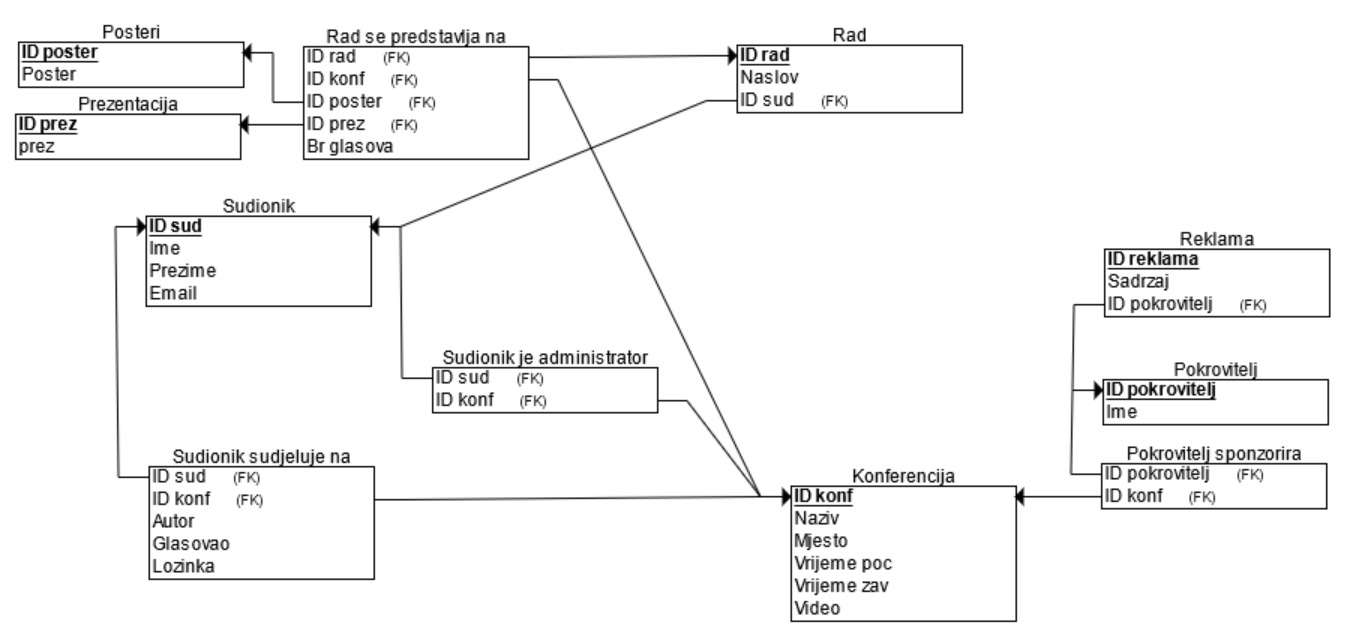
\includegraphics[width=15cm]{slike/dijagram.jpg}
	\caption{Slika 4.1: Dijagram baze podataka}
	\label{fig:fer-logo}
\end{figure}
			
			\eject
			
			
		\section{Dijagram razreda}
		
			\textit{Potrebno je priložiti dijagram razreda s pripadajućim opisom. Zbog preglednosti je moguće dijagram razlomiti na više njih, ali moraju biti grupirani prema sličnim razinama apstrakcije i srodnim funkcionalnostima.}\\
			
			\textbf{\textit{dio 1. revizije}}\\
			
			\textit{Prilikom prve predaje projekta, potrebno je priložiti potpuno razrađen dijagram razreda vezan uz \textbf{generičku funkcionalnost} sustava. Ostale funkcionalnosti trebaju biti idejno razrađene u dijagramu sa sljedećim komponentama: nazivi razreda, nazivi metoda i vrste pristupa metodama (npr. javni, zaštićeni), nazivi atributa razreda, veze i odnosi između razreda.}\\
			
			\textbf{\textit{dio 2. revizije}}\\			
			
			\textit{Prilikom druge predaje projekta dijagram razreda i opisi moraju odgovarati stvarnom stanju implementacije}
			
			
			
			\eject
		
		\section{Dijagram stanja}
			
			
			\textbf{\textit{dio 2. revizije}}\\
			
			\textit{Potrebno je priložiti dijagram stanja i opisati ga. Dovoljan je jedan dijagram stanja koji prikazuje \textbf{značajan dio funkcionalnosti} sustava. Na primjer, stanja korisničkog sučelja i tijek korištenja neke ključne funkcionalnosti jesu značajan dio sustava, a registracija i prijava nisu. }
			
			
			\eject 
		
		\section{Dijagram aktivnosti}
			
			\textbf{\textit{dio 2. revizije}}\\
			
			 \textit{Potrebno je priložiti dijagram aktivnosti s pripadajućim opisom. Dijagram aktivnosti treba prikazivati značajan dio sustava.}
			
			\eject
		\section{Dijagram komponenti}
		
			\textbf{\textit{dio 2. revizije}}\\
		
			 \textit{Potrebno je priložiti dijagram komponenti s pripadajućim opisom. Dijagram komponenti treba prikazivati strukturu cijele aplikacije.}